% 92-21(92쪽) — 원에 내접하는 사각형 ABCD(원문 「오른쪽 그림」). 스캔 화질이 낮아 TikZ 로 다시 그림.
% 라벨은 원문 것만: 꼭짓점 A·B·C·D, 길이 10·2. 선분 BD 의 길이(답)는 그림에 적지 않는다.
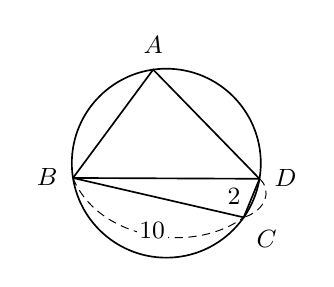
\begin{tikzpicture}[line width=0.6pt, x=0.60cm, y=0.60cm]
  \coordinate (A) at (-0.278,1.981);
  \coordinate (B) at (-1.975,-0.313);
  \coordinate (C) at (1.638,-1.147);
  \coordinate (D) at (1.973,-0.330);
  \draw (0,0) circle [radius=2];
  \draw (B) -- (A) -- (D);
  \draw (B) -- (D);
  \draw (B) -- (C) -- (D);
  % 길이 표시의 점선 호
  \draw[densely dashed, line width=0.35pt] (B) .. controls (-1.45,-1.60) and (0.55,-1.95) .. (C);
  \draw[densely dashed, line width=0.35pt] (D) .. controls (2.24,-0.56) and (2.12,-1.00) .. (C);
  \node[font=\small, anchor=south] at (-0.278,2.10) {$\pt{A}$};
  \node[font=\small, anchor=east] at (-2.09,-0.30) {$\pt{B}$};
  \node[font=\small, anchor=north west] at (1.70,-1.21) {$\pt{C}$};
  \node[font=\small, anchor=west] at (2.08,-0.31) {$\pt{D}$};
  \node[font=\small, fill=white, inner sep=1pt] at (-0.30,-1.42) {$10$};
  \node[font=\small, anchor=east] at (1.78,-0.70) {$2$};
\end{tikzpicture}
